\documentclass[letter]{article}
\renewcommand{\baselinestretch}{1.25}

\usepackage[margin=1in]{geometry}
\usepackage{physics}
\usepackage{amsmath}
\usepackage{graphicx}
\usepackage{hyperref}


% MATLAB Formating Code
\usepackage[numbered,framed]{matlab-prettifier}
\lstset{style=Matlab-editor,columns=fullflexible}
\renewcommand{\lstlistingname}{Script}
\newcommand{\scriptname}{\lstlistingname}

\allowdisplaybreaks

%opening
\title{MECH 6313 - Homework 1}
\author{Jonas Wagner}
\date{2021, February 1}

\begin{document}

\maketitle


\section{Problem 1 - Duffing's Equation}
Duffings Equation is exhibits chaotic behavior with certain parameters. It is discribed by the following:
\begin{displaymath}
	\ddot{y} + \delta \dot{y} - y + y^3 = \alpha \cos(\omega_t t)
\end{displaymath}

\textbf{Problem:}
Simulate the equation for $\delta = 0.05, \alpha = 0.4$, and $\omega_t = 1.3$.\\

\textbf{Solution:}
In matlab the nlsys class (something I have been developing to help in nonlin system simulation - \href{https://github.com/jonaswagner2826/nlsys}{https://github.com/jonaswagner2826/nlsys}) was used to simulate the system and plot the following phase plots and time responses. The MATLAB code for this assignment is available in \appendixname \ref{script:HW1}\\



\begin{figure}[h]
	\centering
	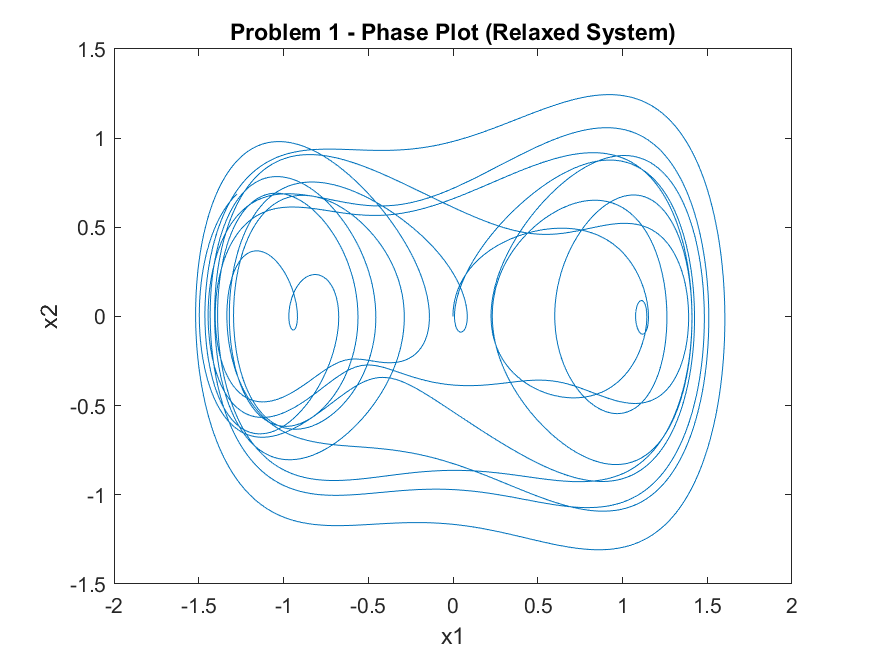
\includegraphics[width=0.7\linewidth]{fig/pblm1_phase}
	\caption{Phase Plot for the Relaxed System}
	\label{fig:pblm1phase}
\end{figure}


\begin{figure}[p]
	\centering
	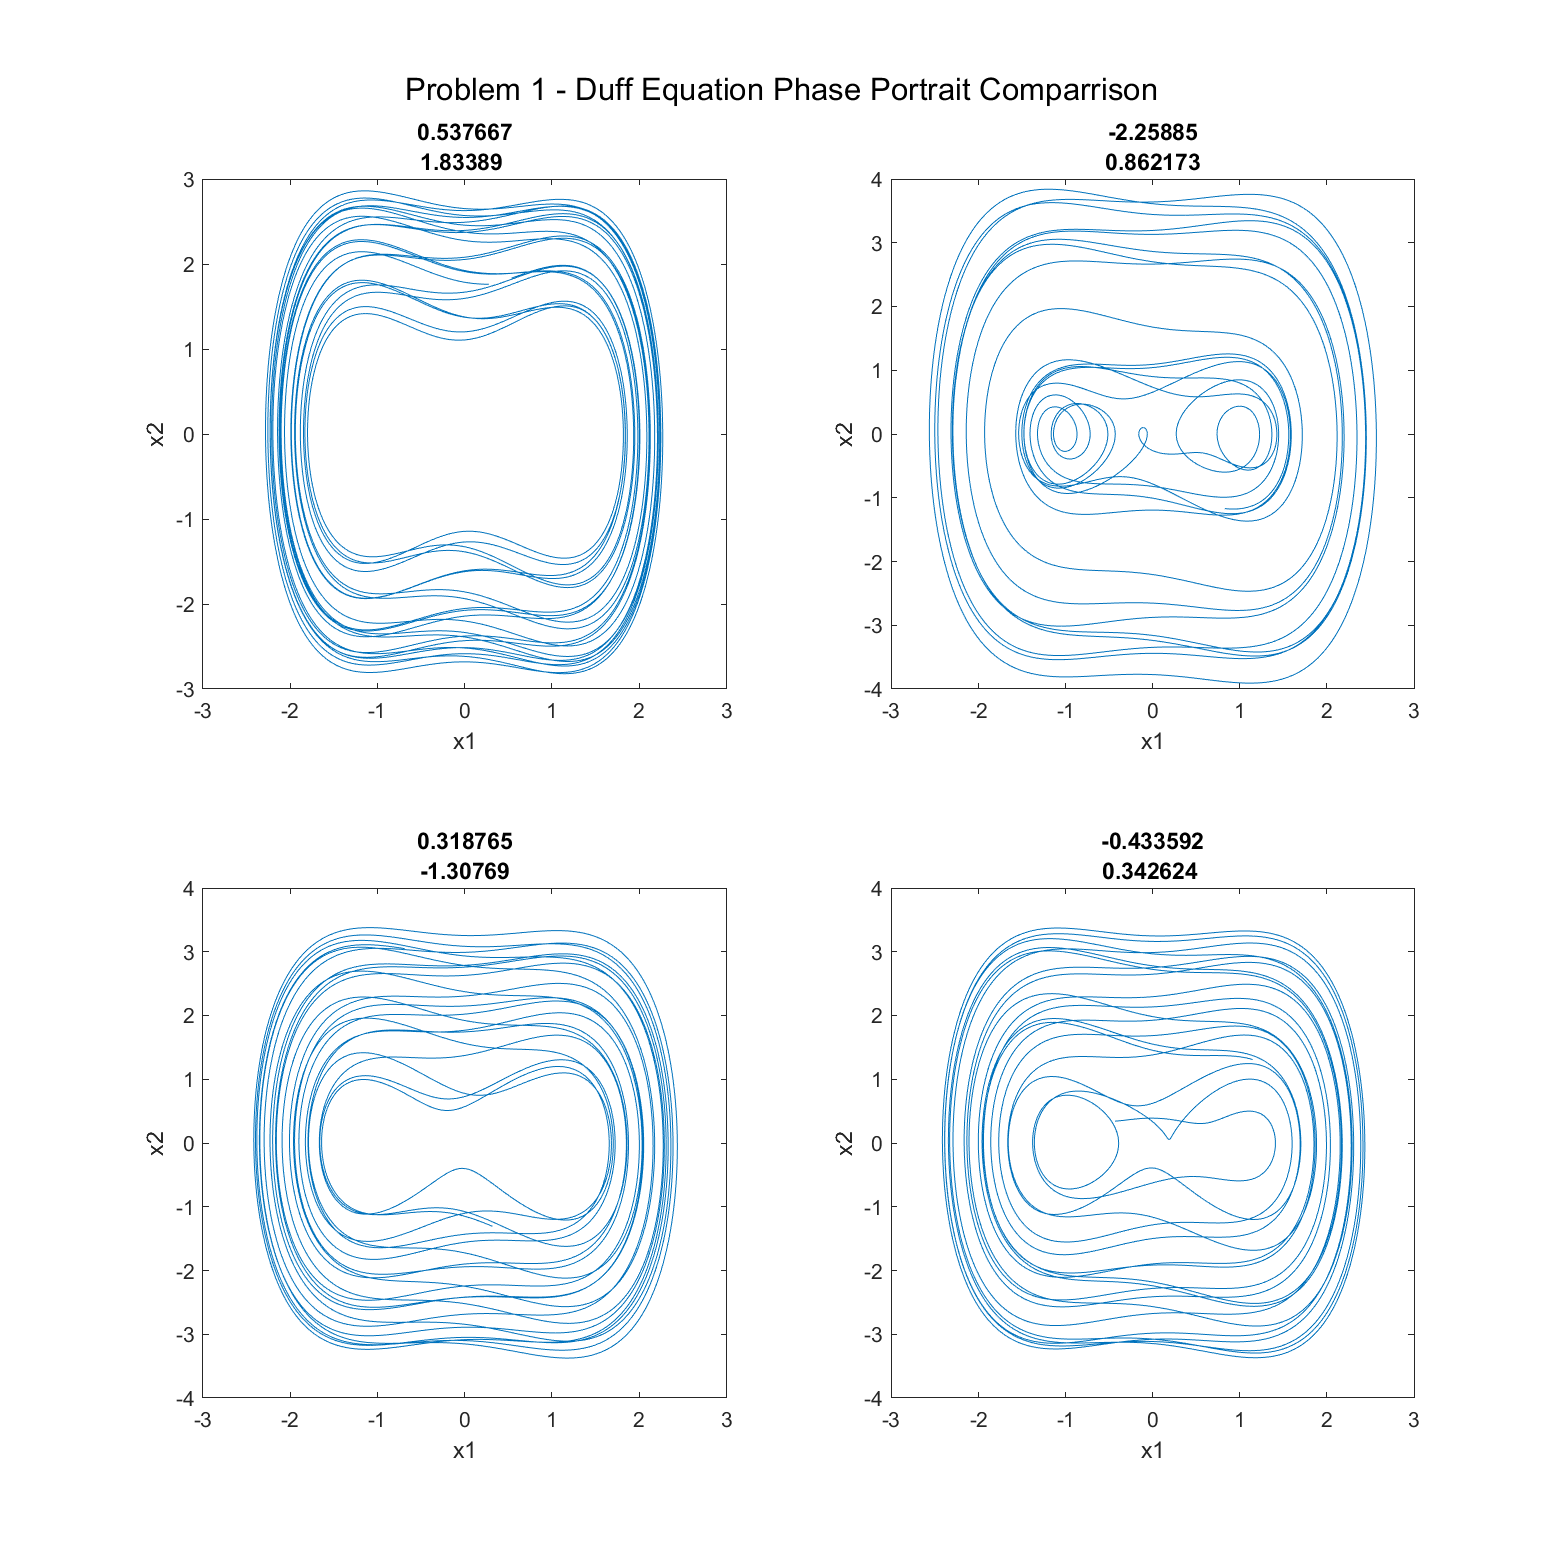
\includegraphics[width=1\linewidth]{fig/pblm1_phase_comparrision}
	\caption{Phase Plot for multiple initial conditions}
	\label{fig:pblm1phasecomparrision}
\end{figure}

\newpage
\begin{figure}[t]
	\centering
	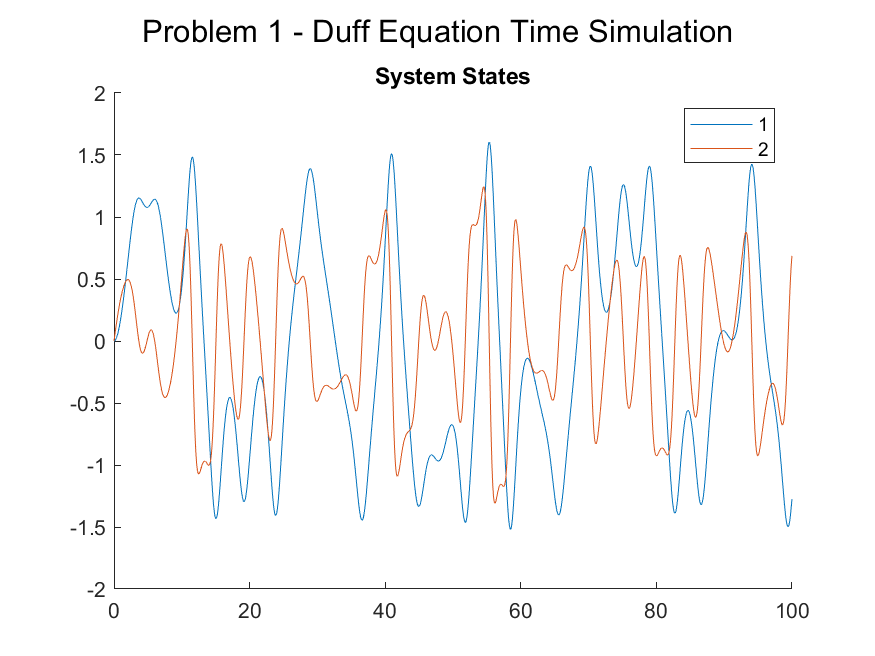
\includegraphics[width=0.8\linewidth]{fig/pblm1_vs_time}
	\caption{Plot of the relaxed system vs time}
	\label{fig:pblm1vstime}
\end{figure}


\textbf{Discussion:}\\

Both the phase portraits and time response of the Duffings equation indicate a fairly chaotic behavior, however it does appear to contentiously rotate around the origin in a periodic fashion (possibly due to the sinusoidal input). Either way, it is difficult to recognize a predictable behavior, and neither decays or explodes predictably.


\newpage
\section{Problem 2 - Van Der Pol Equations}
\textbf{Problem:}
The van der Pole equation is as follows:
\begin{displaymath}
	\ddot{y} + \qty(y^2 - 1)*\dot{y} + y = 0
\end{displaymath}

Plot the phase portrait, time dependence and compare with the response of Duffing's equations.\\

\textbf{Solution:}
In matlab the nlsys class (something I have been developing to help in nonlin system simulation - \href{https://github.com/jonaswagner2826/nlsys}{https://github.com/jonaswagner2826/nlsys}) was used to simulate the system and plot the following phase plots and time responses. The MATLAB code for this assignment is available in \appendixname \ref{script:HW1}

\subsection{Van Der Pol Simulation}

\subsubsection{Phase Portraits}

\begin{figure}[h]
	\centering
	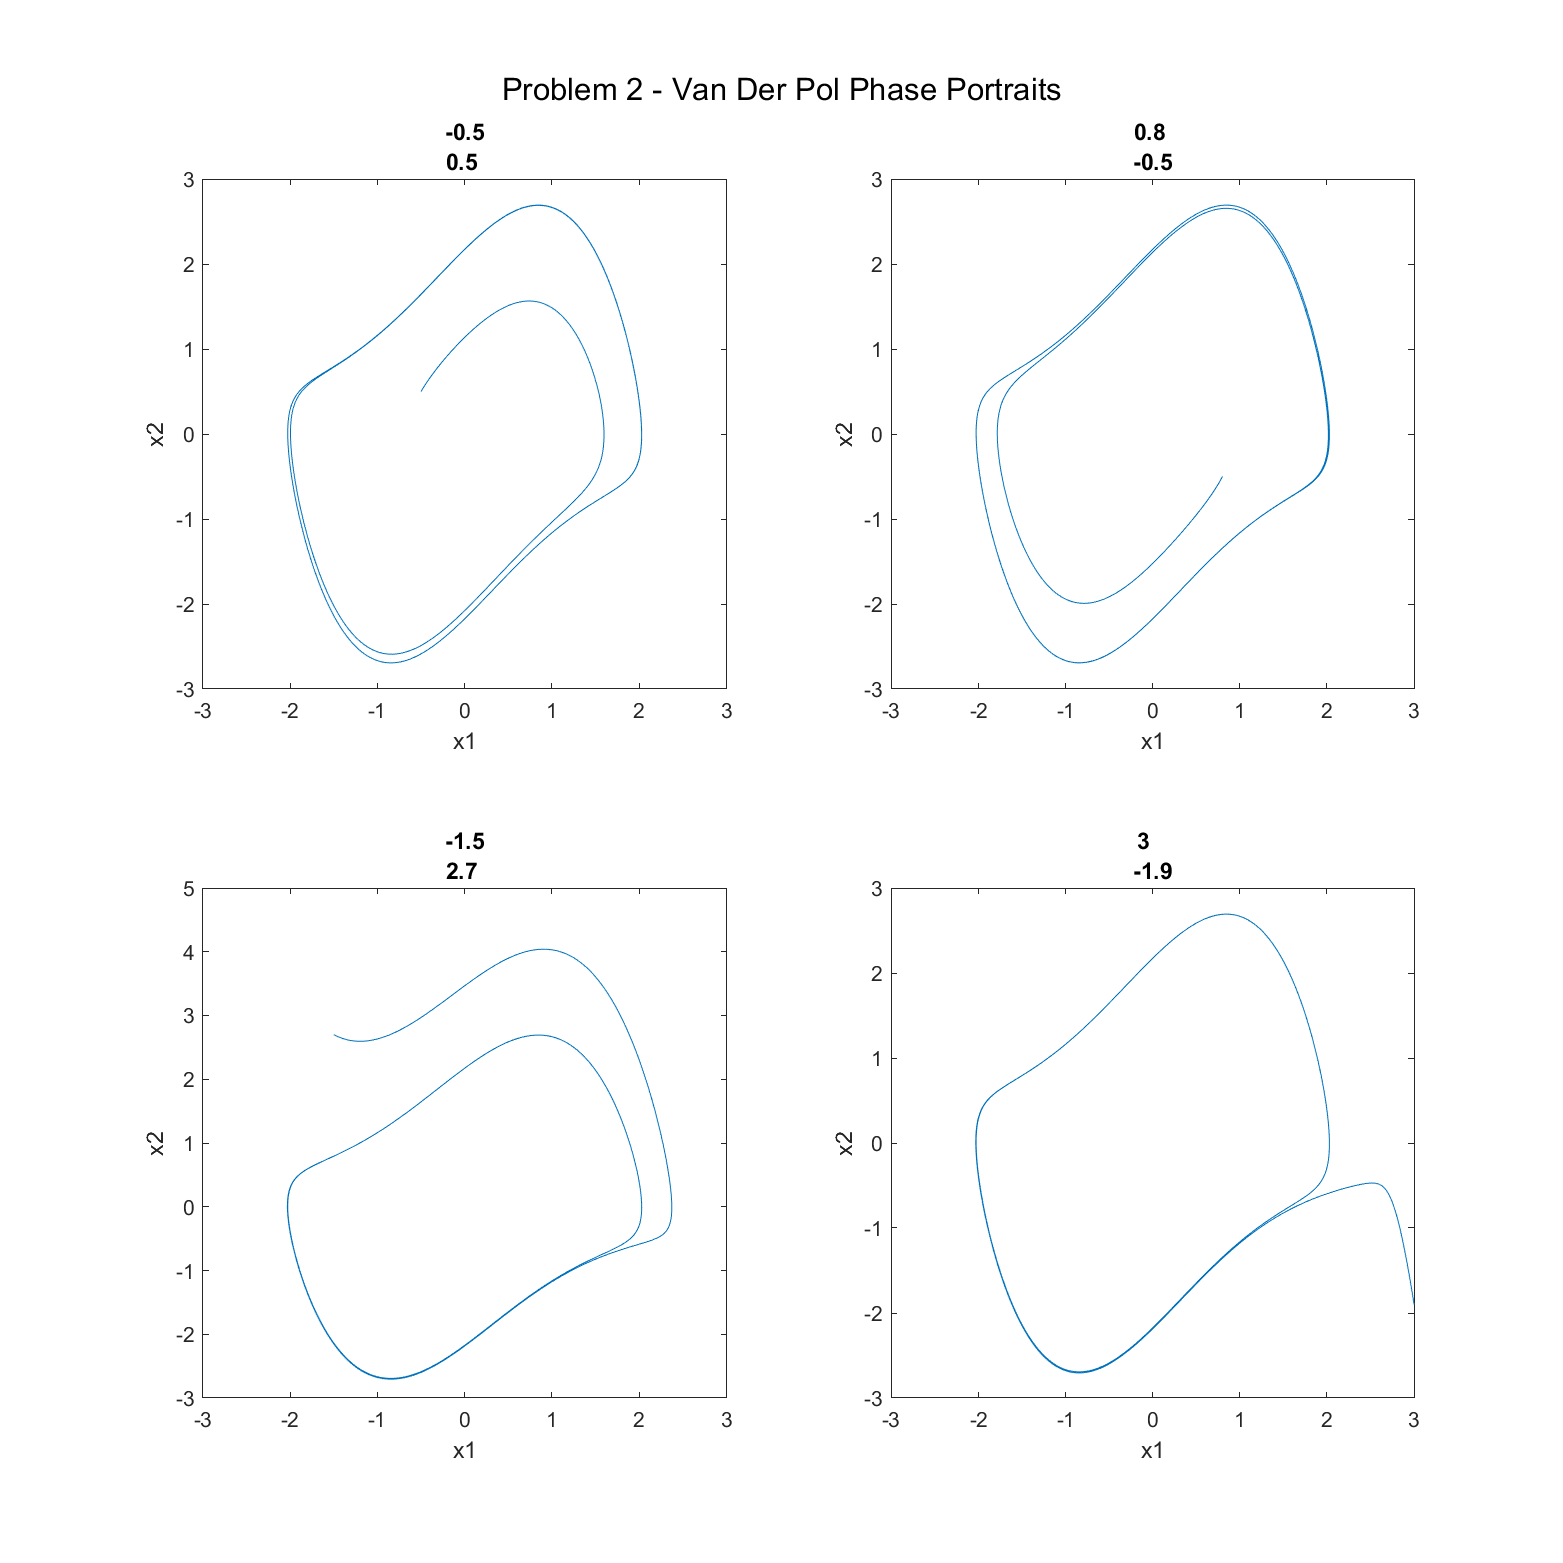
\includegraphics[width=0.8\linewidth]{fig/pblm2_phase_comparrision}
	\caption{Phase Plot for multiple initial conditions}
	\label{fig:pblm2phasecomparrision}
\end{figure}

\newpage
\subsubsection{Time Response}
\begin{figure}[h]
	\centering
	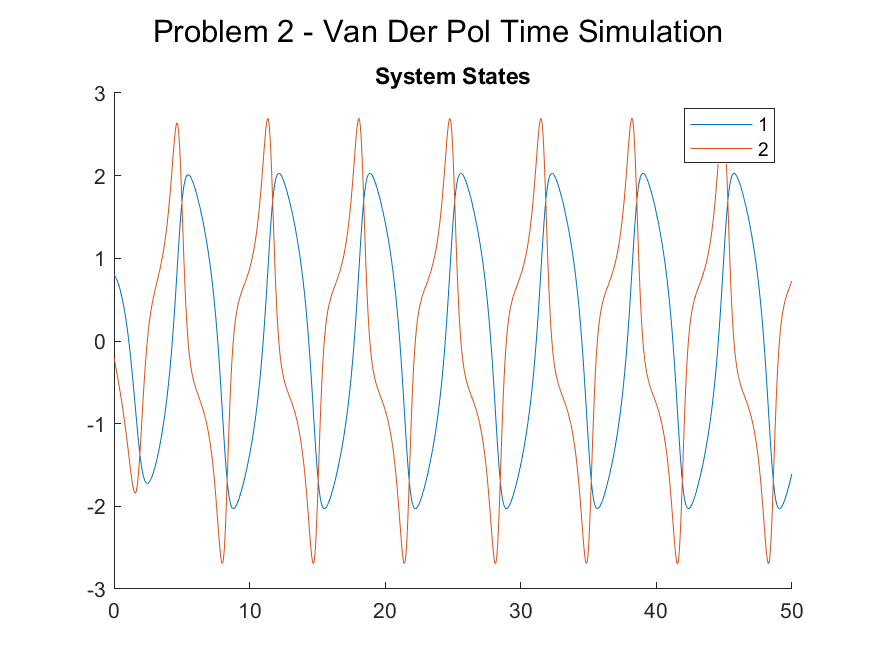
\includegraphics[width=0.8\linewidth]{fig/pblm2_vs_time}
	\caption{Phase Plot for multiple initial conditions}
	\label{fig:pblm2vstime}
\end{figure}


\textbf{Discussion:}

Unlike the results from the duffings equation, the Van Der Pol equations produce a very predictable response. Outside of the equilibrium point located at the origin, the unforced response from any initial equation appears to decay to the exact same periodic motion. Looking at the time response plot, the system states demonstrate a periodic response consistant with expectations from the phase portrait.



\newpage
\subsection{Negative Van Der Pole Equation}

Modifying the nonlinear term of the van der pole equations results in the following differential equation:
\begin{displaymath}
	\ddot{y} - \qty(y^2 - 1)*\dot{y} + y = 0
\end{displaymath}


\subsubsection{System Stability at the Origin}

The Van Der Pol equation can be linearized at the origin by using a taylor's series expansion of the state-space model. The first term can be found by taking the jacobian and evaluating it with $x=\mqty[0&0]^T$.

Letting $x_1 = y$ and $x_2 = \dot{y}$, the following state-space model is derived:
\begin{displaymath}
	\vb{\dot{x}} = f(\vb{x},\vb{u}) = \mqty[x_2 \\ -(x_1^2 - 1) x_2 - x_1]
\end{displaymath}

The jacobians for the $A$ matrix can then be found as:
\begin{align*}
	A 	&= \eval{\mqty[\dv{f_1}{x_1}& \dv{f_1}{x_2}\\ \dv{f_2}{x_1} & \dv{f_2}{x_2}]}_{\vb{x}= \vb{x}_0}\\
		&= \eval{\mqty[0 & 1\\ -2 x_1 x_2 -1 & -x_1^2 +1]}_{\vb{x} = \vb{x}_0}\\
		&= \mqty[0 & 1 \\ -1 &1]
\end{align*}

The stability of this matrix can then be determined by looking at the eigenvalues:
\begin{displaymath}
	\Lambda\{A\} = 0.5 \pm j 0.866
\end{displaymath}

Since $\real\{\Lambda\{A\}\} > 0$, the linearized system is said to be unstable at the origin.

\newpage
\subsubsection{Phase Portraits}

\begin{figure}[h]
	\centering
	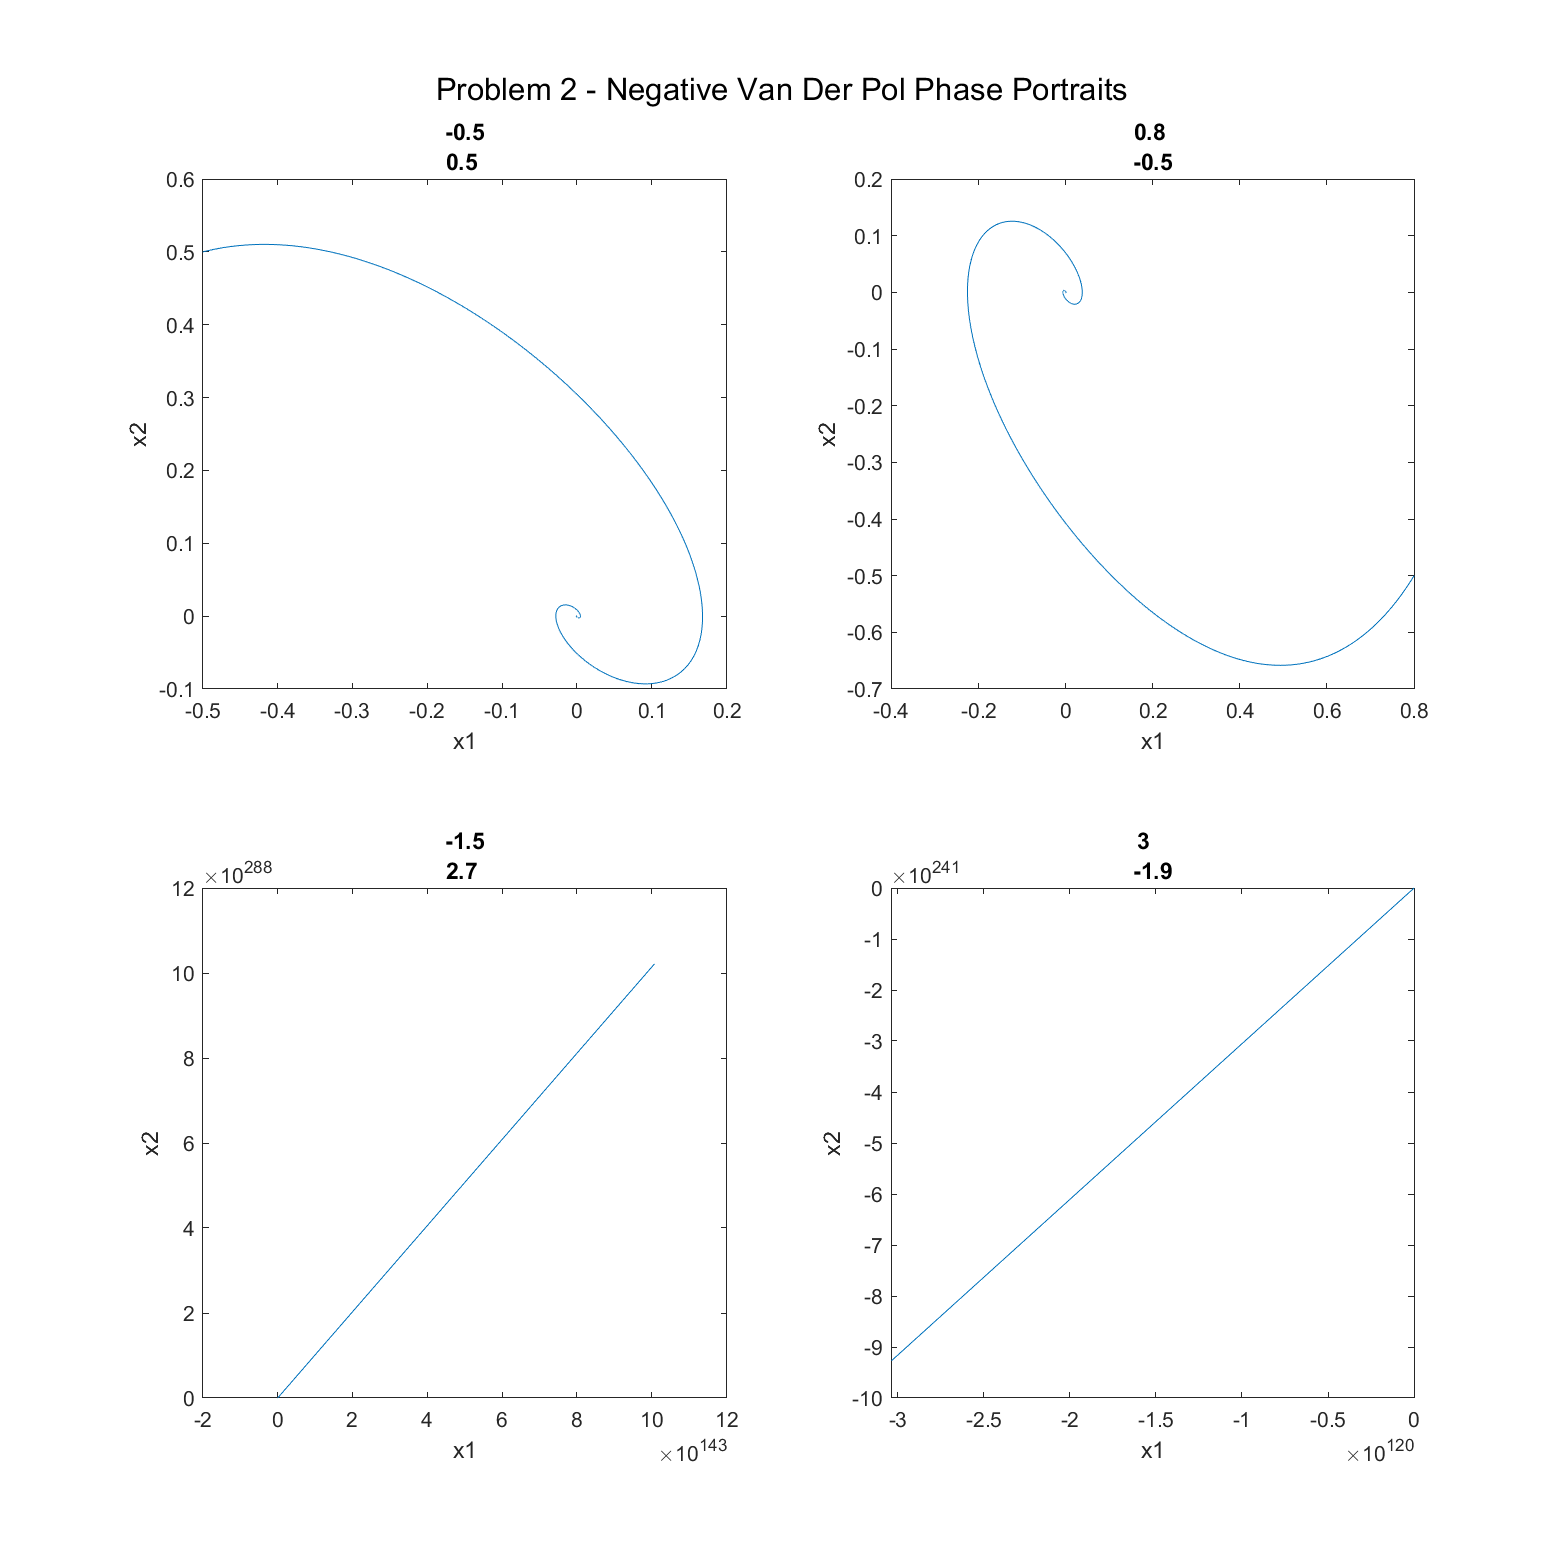
\includegraphics[width=1\linewidth]{fig/pblm2_phase_comparrision_neg}
	\caption{Phase Plot for multiple initial conditions}
	\label{fig:pblm2phasecomparrisionneg}
\end{figure}

\newpage
\subsubsection{Time Response}
\begin{figure}[h]
	\centering
	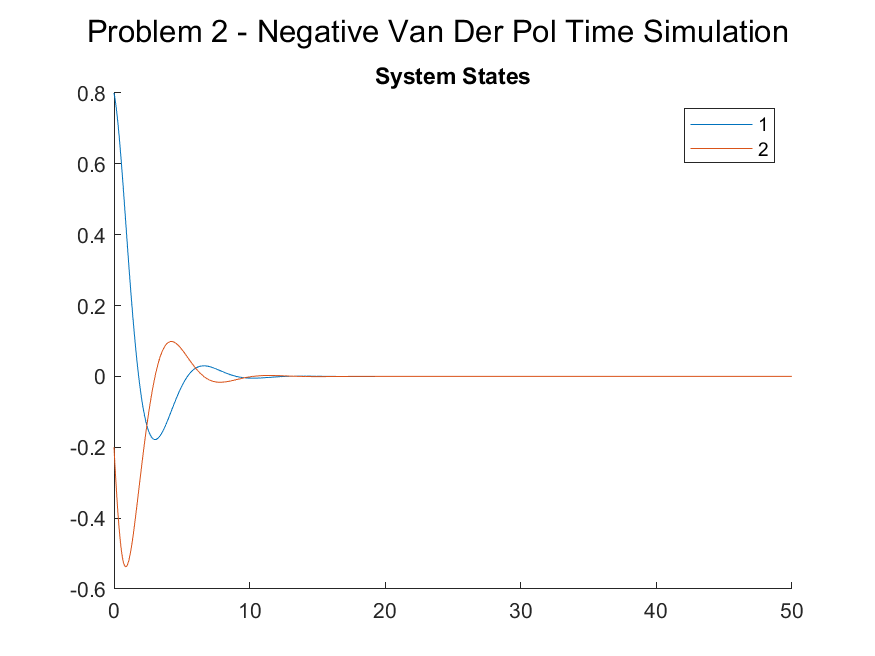
\includegraphics[width=0.8\linewidth]{fig/pblm2_vs_time_neg}
	\caption{Phase Plot for multiple initial conditions}
	\label{fig:pblm2vstimeneg}
\end{figure}


\textbf{Discussion:}
Unlike in the positive van der pol equation, when the nonlinear term is set to be negative it reacts almost directly oposite of the positive one. As was discovered, the origin within the negative system is asymptotically stable, but this is not true in general. From the simulations it is apparent that the same boundary that is the steady-state response for the positve van der pol equation is the boundary of instability. The system is indead localy stable within that boundary and decays to zero, but outside it blows up. It actually doesn't blow up exactly as expected either, depending on the initial condition it won't necessarily just explode out to the extremes of its own quadrant but instead it changes with the initial condition.







\newpage
\section{Problem 3 - Magnetic  Suspension System}
	An electromagnet suspends a ball and is controlled by a feedback system based on the measured postion. The equation of motion for the ball is given as:
	
	\begin{equation} \label{eq:ball_eq}
		m \ddot{y} = -k \dot{y} + mg + F(y,i)
	\end{equation}

	where $m$ is the mass of the ball, $y \geq 0$ is the vertical position of the ball relative to the electro magnet, $k$ is the friction coeficent, $g$ is the accelleration of gravity, and $F(y,i)$ is the force generated by the magnet dependent on the position and current ($i$).\\
	
	The inductance of the electromagnet is given as a function of the ball's position as:
	\begin{equation}\label{eq:L_def}
		L(y) = L_1 + \frac{L_0}{1 + y/a}
	\end{equation}
	where $L_1, L_0, a > 0$.\\
	
	The energy stored within the electromagnet is given as a function of inductance:
	\begin{equation}\label{eq:E_def}
		E(y,i) = \frac{1}{2} L(y) i^2 = \frac{1}{2} \qty(L_1 + \frac{L_0}{1 + y/a}) i^2
	\end{equation}
	
	The force on the ball is then calculated as the derivative of energy with respect to position:
	\begin{equation}\label{eq:F_def}
		F(y,i) = \pdv{E}{y} = \frac{- L_0 i^2}{2 a (1+y/a)^2}
	\end{equation}
	
	The electric circuit controlling the electro magnet is governed by KVL as:
	\begin{equation}\label{eq:KVL_eq}
		v = \dot{\phi} + R i
	\end{equation}
	where $v$ is the input voltage, $R$ is the resistance and $\phi = L(y) i$.
	
	
	\begin{figure}[h]
		\centering
		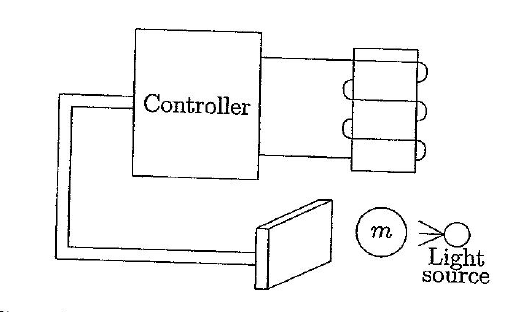
\includegraphics[width=0.5\linewidth]{fig/pblm6_diagram}
		\caption{Magnetic suspension system diagram}
		\label{fig:pblm6diagram}
	\end{figure}


\newpage
\subsection{State Space Model}

Let the following state variables be defined:
$$x_1 = y \hspace{1in} x_2 = \dot{y} \hspace{1in} x_3 = i \hspace{1in} u = v$$

\begin{equation}\label{eq:state_vars}
	\centering
	\vb{x} = \mqty[x_1\\ x_2\\ x3] = \mqty[y\\ \dot{y} \\ i] \hspace{1in} \vb{u} = \mqty[u] = \mqty[v]
\end{equation}

From the definition, the following state equation can be stated directly:
\begin{equation}\label{eq:x1_dot_def}
	\dot{x}_1 = x_2
\end{equation}

A second equation of motion can be derived from \eqref{eq:ball_eq} and \eqref{eq:F_def}:
\begin{align}
	\ddot{y}	&= -\qty(\frac{k}{m}) \ \dot{y} + g + \frac{1}{m} F(y,i)\nonumber \\
				&= -\qty(\frac{k}{m}) \dot{y} + g + \frac{1}{m} \ \cfrac{- L_0 \qty(i)^2}{2 a (1+y/a)^2} \nonumber \\
	\dot{x}_2	&= -\qty(\frac{k}{m}) x_2 + g + \cfrac{- L_0 \qty(x_3)^2}{2 a m \qty(1 + \frac{x_1}{a})^2}
\end{align}

From \eqref{eq:KVL_eq} the following can be derived:
\begin{align}
	v 	&= \pdv{t} \qty(L(y) i) + R i\nonumber\\
		&= \qty(\dot{L}(y) i + L(y) \dot{i}) + R i \label{eq:KVL_2}
\end{align}

$\dot{L}(y)$ can be calculated from \eqref{eq:F_def}:
\begin{align}
	\dot{L}(y) 	&= \pdv{t}\qty(L_1 + \frac{L_0}{1 + y/a})\nonumber \\
				&= - \cfrac{L_0 \ a \ \dot{y}}{\qty(a + y)^2} \label{eq:L_dot_def}
\end{align}

Substituting \eqref{eq:F_def} and \eqref{eq:L_dot_def} into \eqref{eq:KVL_2}, the following can be obtained:
\begin{align}
	v	&= - \cfrac{L_0 \ a \ \dot{y} \ i}{\qty(a + y)^2}  + \qty(L_1 + \frac{L_0}{1 + y/a}) \dot{i} + R i \nonumber\\
	\qty(\frac{L_1 \qty(1 + y/a) + L_0}{1 + y/a}) \dot{i} &= \cfrac{L_0 \ a \ \dot{y} \ i}{\qty(a + y)^2} - R i  + v \nonumber \\
	\dot{i} &= \qty(\frac{1 + y/a}{L_1 \qty(1 + y/a) + L_0}) \qty(\cfrac{L_0 \ a \ \dot{y} \ i}{\qty(a + y)^2} - R i + v) \nonumber\\
	\dot{x}_3 &= \qty(\frac{1 + {x_1}/a}{L_1 \qty(1 + {x_1}/a) + L_0}) \qty(\cfrac{L_0 \ a \ {x_2} \ i}{\qty(a + {x_1})^2} - R {x_3} + u) \label{eq:x3_dot_def}
\end{align}


The full state-space model is given as:
\begin{equation}\label{eq:state_space_def}
	\dot{\vb{x}} = \mqty[x_2\\
						-\qty(\frac{k}{m}) x_2 + g + \cfrac{- L_0 \qty(x_3)^2}{2 a m \qty(1 + \frac{x_1}{a})^2}\\
						\qty(\cfrac{1 + {x_1}/a}{L_1 \qty(1 + {x_1}/a) + L_0}) \qty(\cfrac{L_0 \ a \ {x_2} \ i}{\qty(a + {x_1})^2} - R {x_3} + u)]
\end{equation}\\


\subsection{Steady-State Solution}

The steady-state equation will occur when $\dot{x_1} = \dot{x_2} = 0$, so the state-space model can be used to find this condition at a certain position, $r>0$.

Since $\dot{x_1} = 0$ and $y = r$, the following can be defined:
\begin{align}
	x_1 &= y = r \label{eq:x_1_ss}\\
	x_2 &= \dot{x_1} = 0 \label{eq:x_2_ss}
\end{align}

$L_{ss}(r)$ is then calculated from \eqref{eq:L_def}:
\begin{equation} \label{eq:L_ss}
	L_{ss}(r) =  L_1 + \frac{L_0}{1 + r/a}
\end{equation}

Similarly, $\dot{L}_{ss}(r)$ is then calculated from \eqref{eq:L_dot_def}:
\begin{equation}\label{eq:L_dot_ss}
	\dot{L}_{ss}(r) = - \cfrac{L_0 \ a \ (0)}{\qty(a + r)^2} = 0
\end{equation}

Referring back to \eqref{eq:KVL_2}, $v$ and $i$ can be related by the following:
\begin{align}
	v 	&= \qty(\dot{L}(y) i + L(y) \dot{i}) + R i \nonumber \\
		&= \qty((0) i + \qty(L_1 + \frac{L_0}{1 + r/a}) \dot{i}) + R i \nonumber \\
		&= \qty(L_1 + \frac{L_0}{1 + r/a}) \dot{i} + R i \label{eq:KVL_3}\\
	\intertext{If you make the assumption that $I_{ss}$ is a constant (something I don't believe),}
	V_{ss}	&= R I_{ss}\\
	I_{ss}	&= \frac{V_{ss}}{R} \label{eq:I_V_ss_rel}
\end{align}

In this case, $F_{ss}$ can be calculated from \eqref{eq:F_def} and \eqref{eq:I_V_ss_rel}:
\begin{align}
	F_{ss} 	&= \frac{- L_0 \qty(\frac{V_{ss}}{R})^2}{2 a \qty(1+r/a)^2} \nonumber \\
			&= \frac{- L_0 V_{ss}^2}{2 a R^2 \qty(1+r/a)^2}\label{eq:F_ss_def}
\end{align}

In order to maintain static conditions, $F_ss = - m g$, so $V_{ss}$ can be found as:
\begin{align}
	F_{ss} = mg &= \frac{- L_0 V_{ss}^2}{2 a R^2 \qty(1+r/a)^2}\\
	V_{ss}^2	&= \frac{- 2 a m g R^2 \qty(1+r/a)^2}{L_0}\\
	V_{ss}		&= \sqrt{\qty(\cfrac{-2 a \qty(mg) \qty(R^2)}{L_0}) \qty(1+r/a)^2} \label{eq:V_ss_def}
\end{align}

$I_ss$ is then calculated from \eqref{eq:I_V_ss_rel} and \eqref{eq:V_ss_def}:
\begin{align}
	I_{ss}	&= \frac{1}{R} \sqrt{\qty(\cfrac{-2 a \qty(mg) \qty(R^2)}{L_0}) \qty(1+r/a)^2} \nonumber \\
			&= \sqrt{\qty(\cfrac{-2 a \qty(mg)}{L_0}) \qty(1+r/a)^2} \label{eq:I_ss_def}
\end{align}



\newpage
\section{Problem 4 - Bifurcation Examples}

Additional functionality was added to the nlsys class in order to introduce bifurcation plots.

\subsection{Pblm 3.4.2}

\begin{align*}
	\dot{x} = r x - \sinh(x)
\end{align*}

As is evident in the bifurcation diagram, the pitchfork diagram is supercritical. $r_c$ was found by differentiating $f(x,r)$, solving for $x_c$, substituting back into $f(x,r)$ and then solving for $r_c = 1$.


\begin{figure}[h]
	\centering
	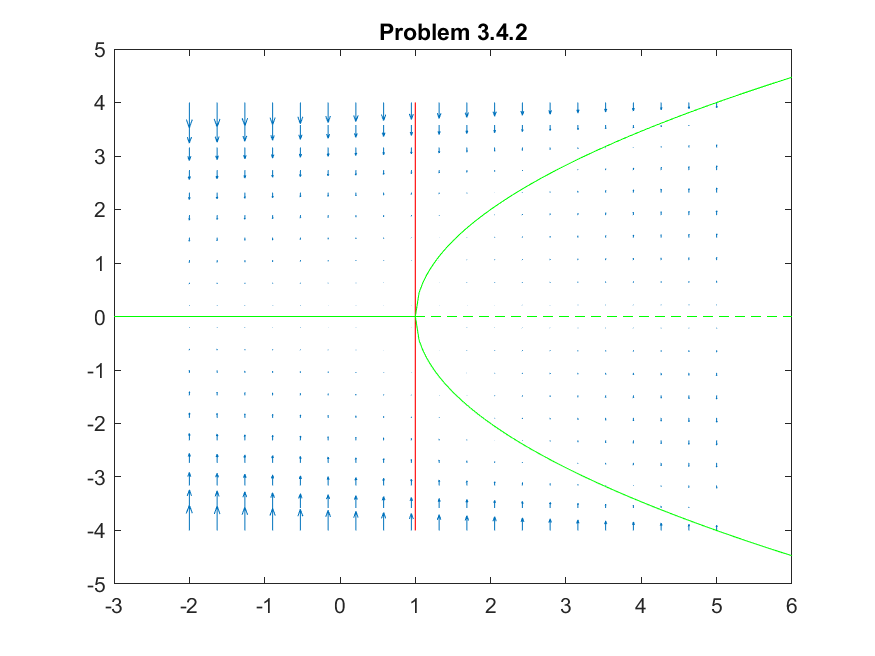
\includegraphics[width=\linewidth]{fig/pblm4_342}
	\caption{Bifurcation Diagram for problem 3.4.2}
	\label{fig:pblm4342}
\end{figure}




\newpage
\subsection{Pblm 3.4.4}

\begin{align*}
	\dot{x} = x + \cfrac{r x}{1+x^2}
\end{align*}

As is evident in the bifurcation diagram, the pitchfork diagram is subcritical. $r_c$ was found by differentiating $f(x,r)$, solving for $x_c$, substituting back into $f(x,r)$ and then solving for $r_c = -1$.


\begin{figure}[h]
	\centering
	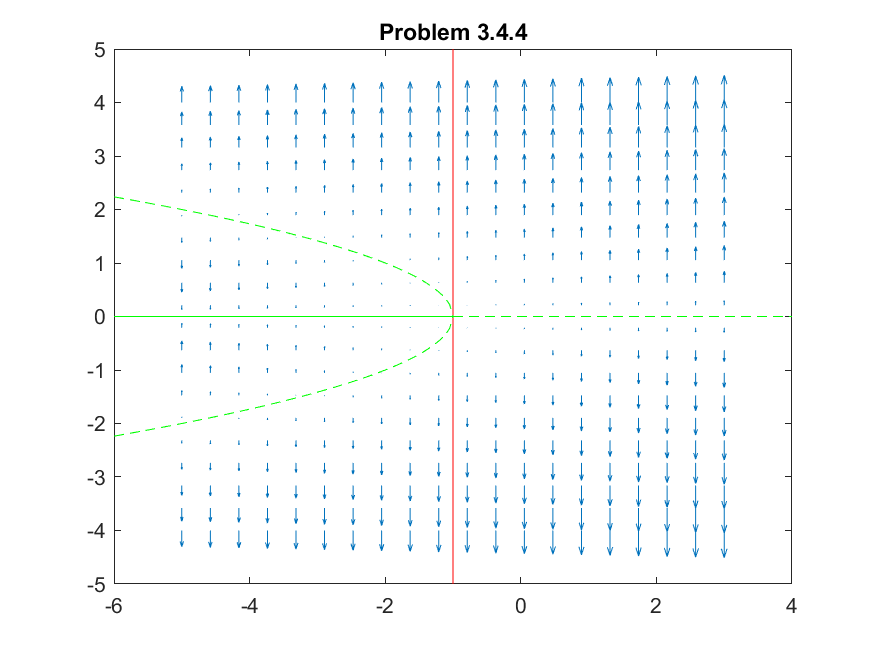
\includegraphics[width=\linewidth]{fig/pblm4_344}
	\caption{Bifurcation Diagram for problem 3.4.4}
	\label{fig:pblm4344}
\end{figure}

\newpage
\subsection{Pblm 3.4.7}

\begin{align*}
	\dot{x} = 5 - r e^{-x^2}
\end{align*}

As is evident in the bifurcation diagram, is a saddle node bifurcation with $r_c = 1$.


\begin{figure}[h]
	\centering
	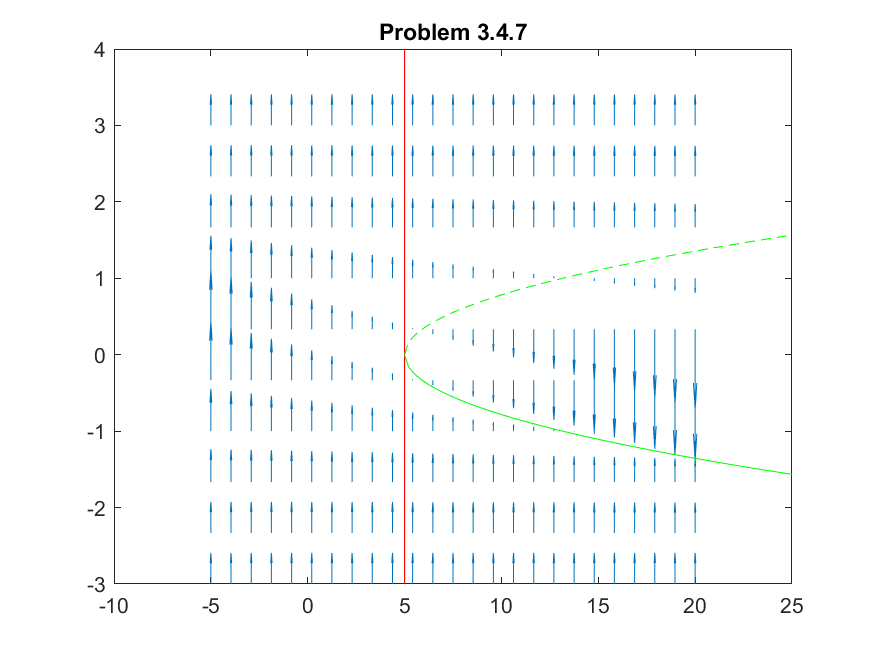
\includegraphics[width=\linewidth]{fig/pblm4_347}
	\caption{Bifurcation Diagram for problem 3.4.7}
	\label{fig:pblm4347}
\end{figure}

\newpage
\subsection{Pblm 3.4.9}

\begin{align*}
	\dot{x} = x + \tanh(rx)
\end{align*}

As is evident in the bifurcation diagram, the pitchfork diagram is subcritical. $r_c$ was found by differentiating $f(x,r)$, solving for $x_c$, substituting back into $f(x,r)$ and then solving for $r_c = -1$.


\begin{figure}[h]
	\centering
	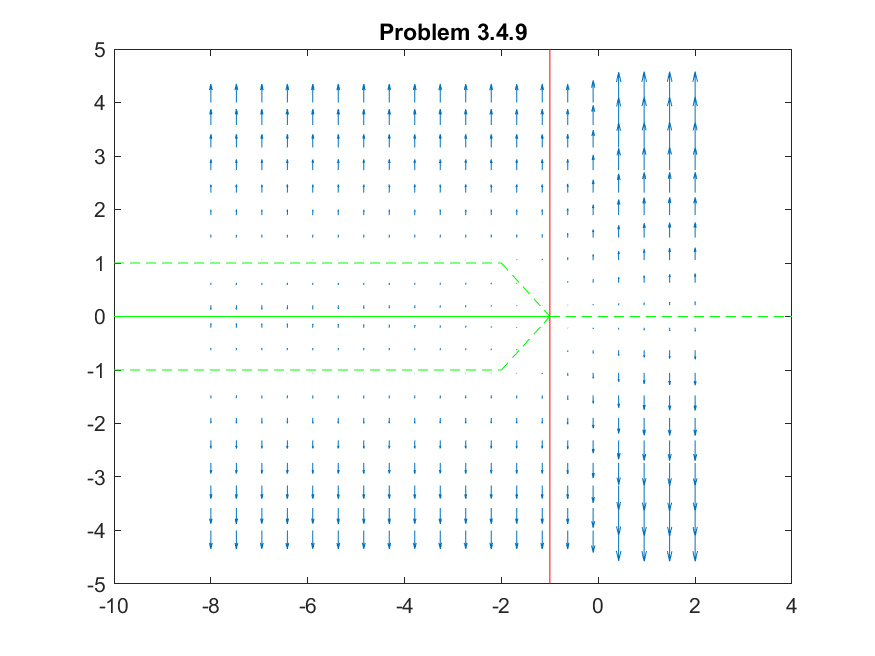
\includegraphics[width=\linewidth]{fig/pblm4_349}
	\caption{Bifurcation Diagram for problem 3.4.9}
	\label{fig:pblm4349}
\end{figure}




\newpage
\appendix
\section{MATLAB Code:}
All code I write in this course can be found on my GitHub repository:\\
\href{https://github.com/jonaswagner2826/MECH6313}{https://github.com/jonaswagner2826/MECH6313}
% MECH6313_HW1
\lstinputlisting[caption={MECH6313\_HW1},label={script:HW1}]{MECH6313_HW1.m}


\end{document}
